\chapter{Этапы формирования обучающей выборки для задачи классификации крюков и знамён}
\section{Подготовка обучающей выборки для нейросетевой модели распознавания крюков и знамён}

Первоначальный этап включал создание шрифта, содержащего крюки и знамёна, с целью обеспечить совместимость 
результатов классификации с современными текстовыми редакторами. Кодирование классов осуществлялось с 
использованием Unicode-символов, соответствующих определённым символам в шрифте (например, Kruk.ttf). %%% тут бы оформить ссыл очку
Это позволяет непосредственно использовать генерируемые классы в текстовых редакторах, таких как Microsoft Word, 
что значительно упрощает процесс внедрения результатов распознавания в практическое применение. 
(см. рис. \ref{pic:Kruk.ttf} \ref{pic:outFont.ttf}).
\begin{figure}[H]
  \begin{center}
    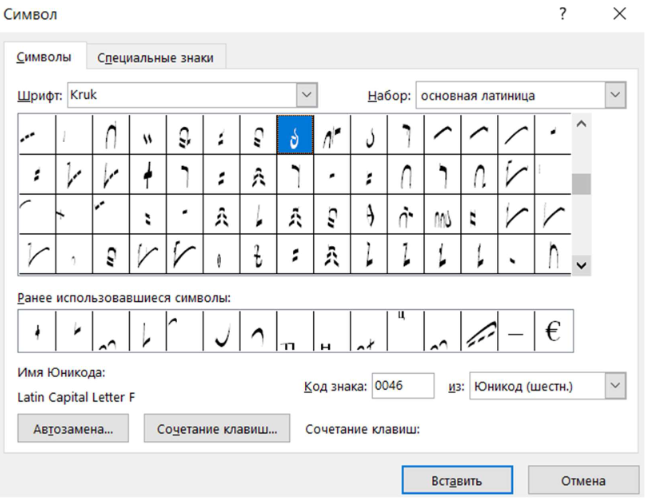
\includegraphics[width=.7\columnwidth]{./img/Kruk.ttf.png}%
  \end{center}
  \caption{Отображение символов в шрифте Kruk.ttf.}%
  \label{pic:Kruk.ttf}%
\end{figure}

\begin{figure}[H]
  \begin{center}
    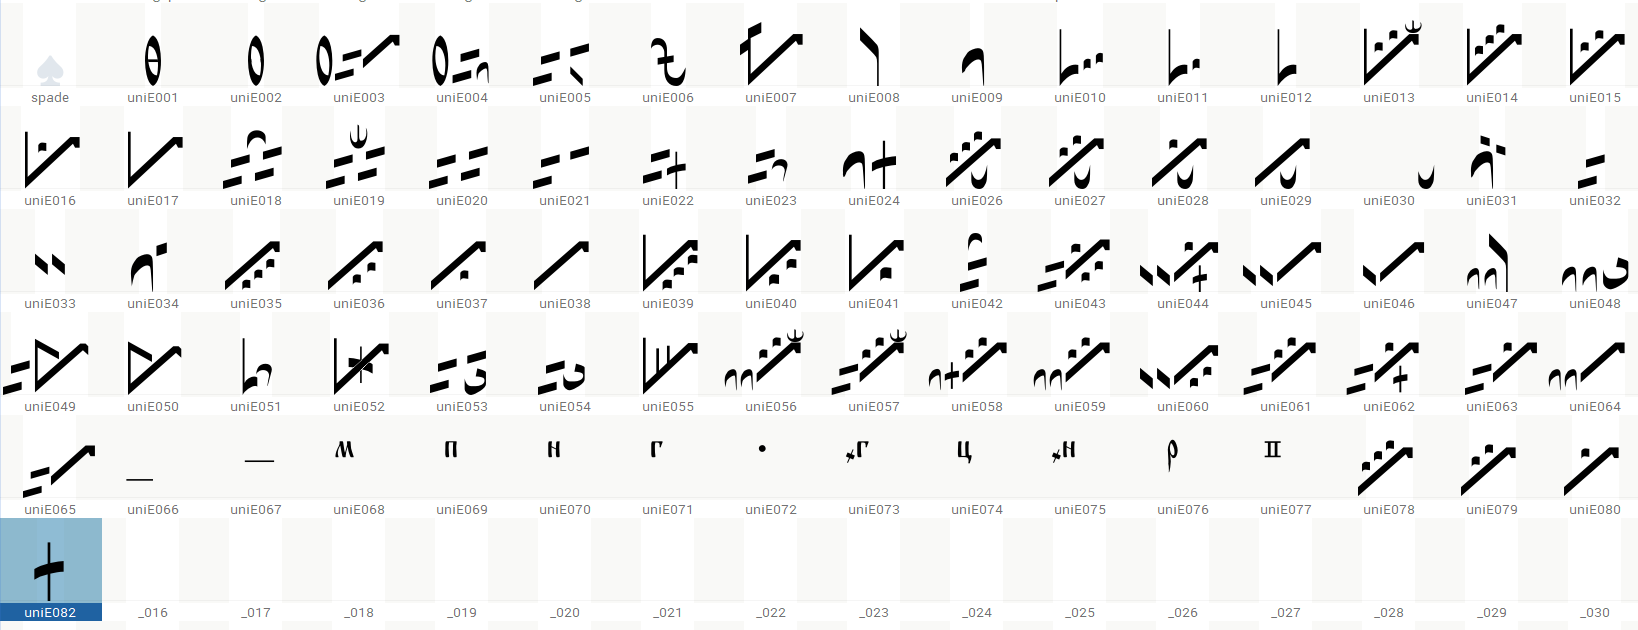
\includegraphics[width=.9\columnwidth]{./img/outFont.ttf.png}%
  \end{center}
  \caption{Классификация крюков в выборке.}%
  \label{pic:outFont.ttf}%
\end{figure}

Для формирования начальной выборки была выбрана рукопись XVII века, известная своим хорошим качеством и 
чёткостью изображений. Процесс предварительной обработки включал бинаризацию страниц рукописи с 
использованием метода Отсу для улучшения контраста и выделения крюков. (см. рис. \ref{pic:binaraize}).
\begin{figure}[H]
  \begin{center}
    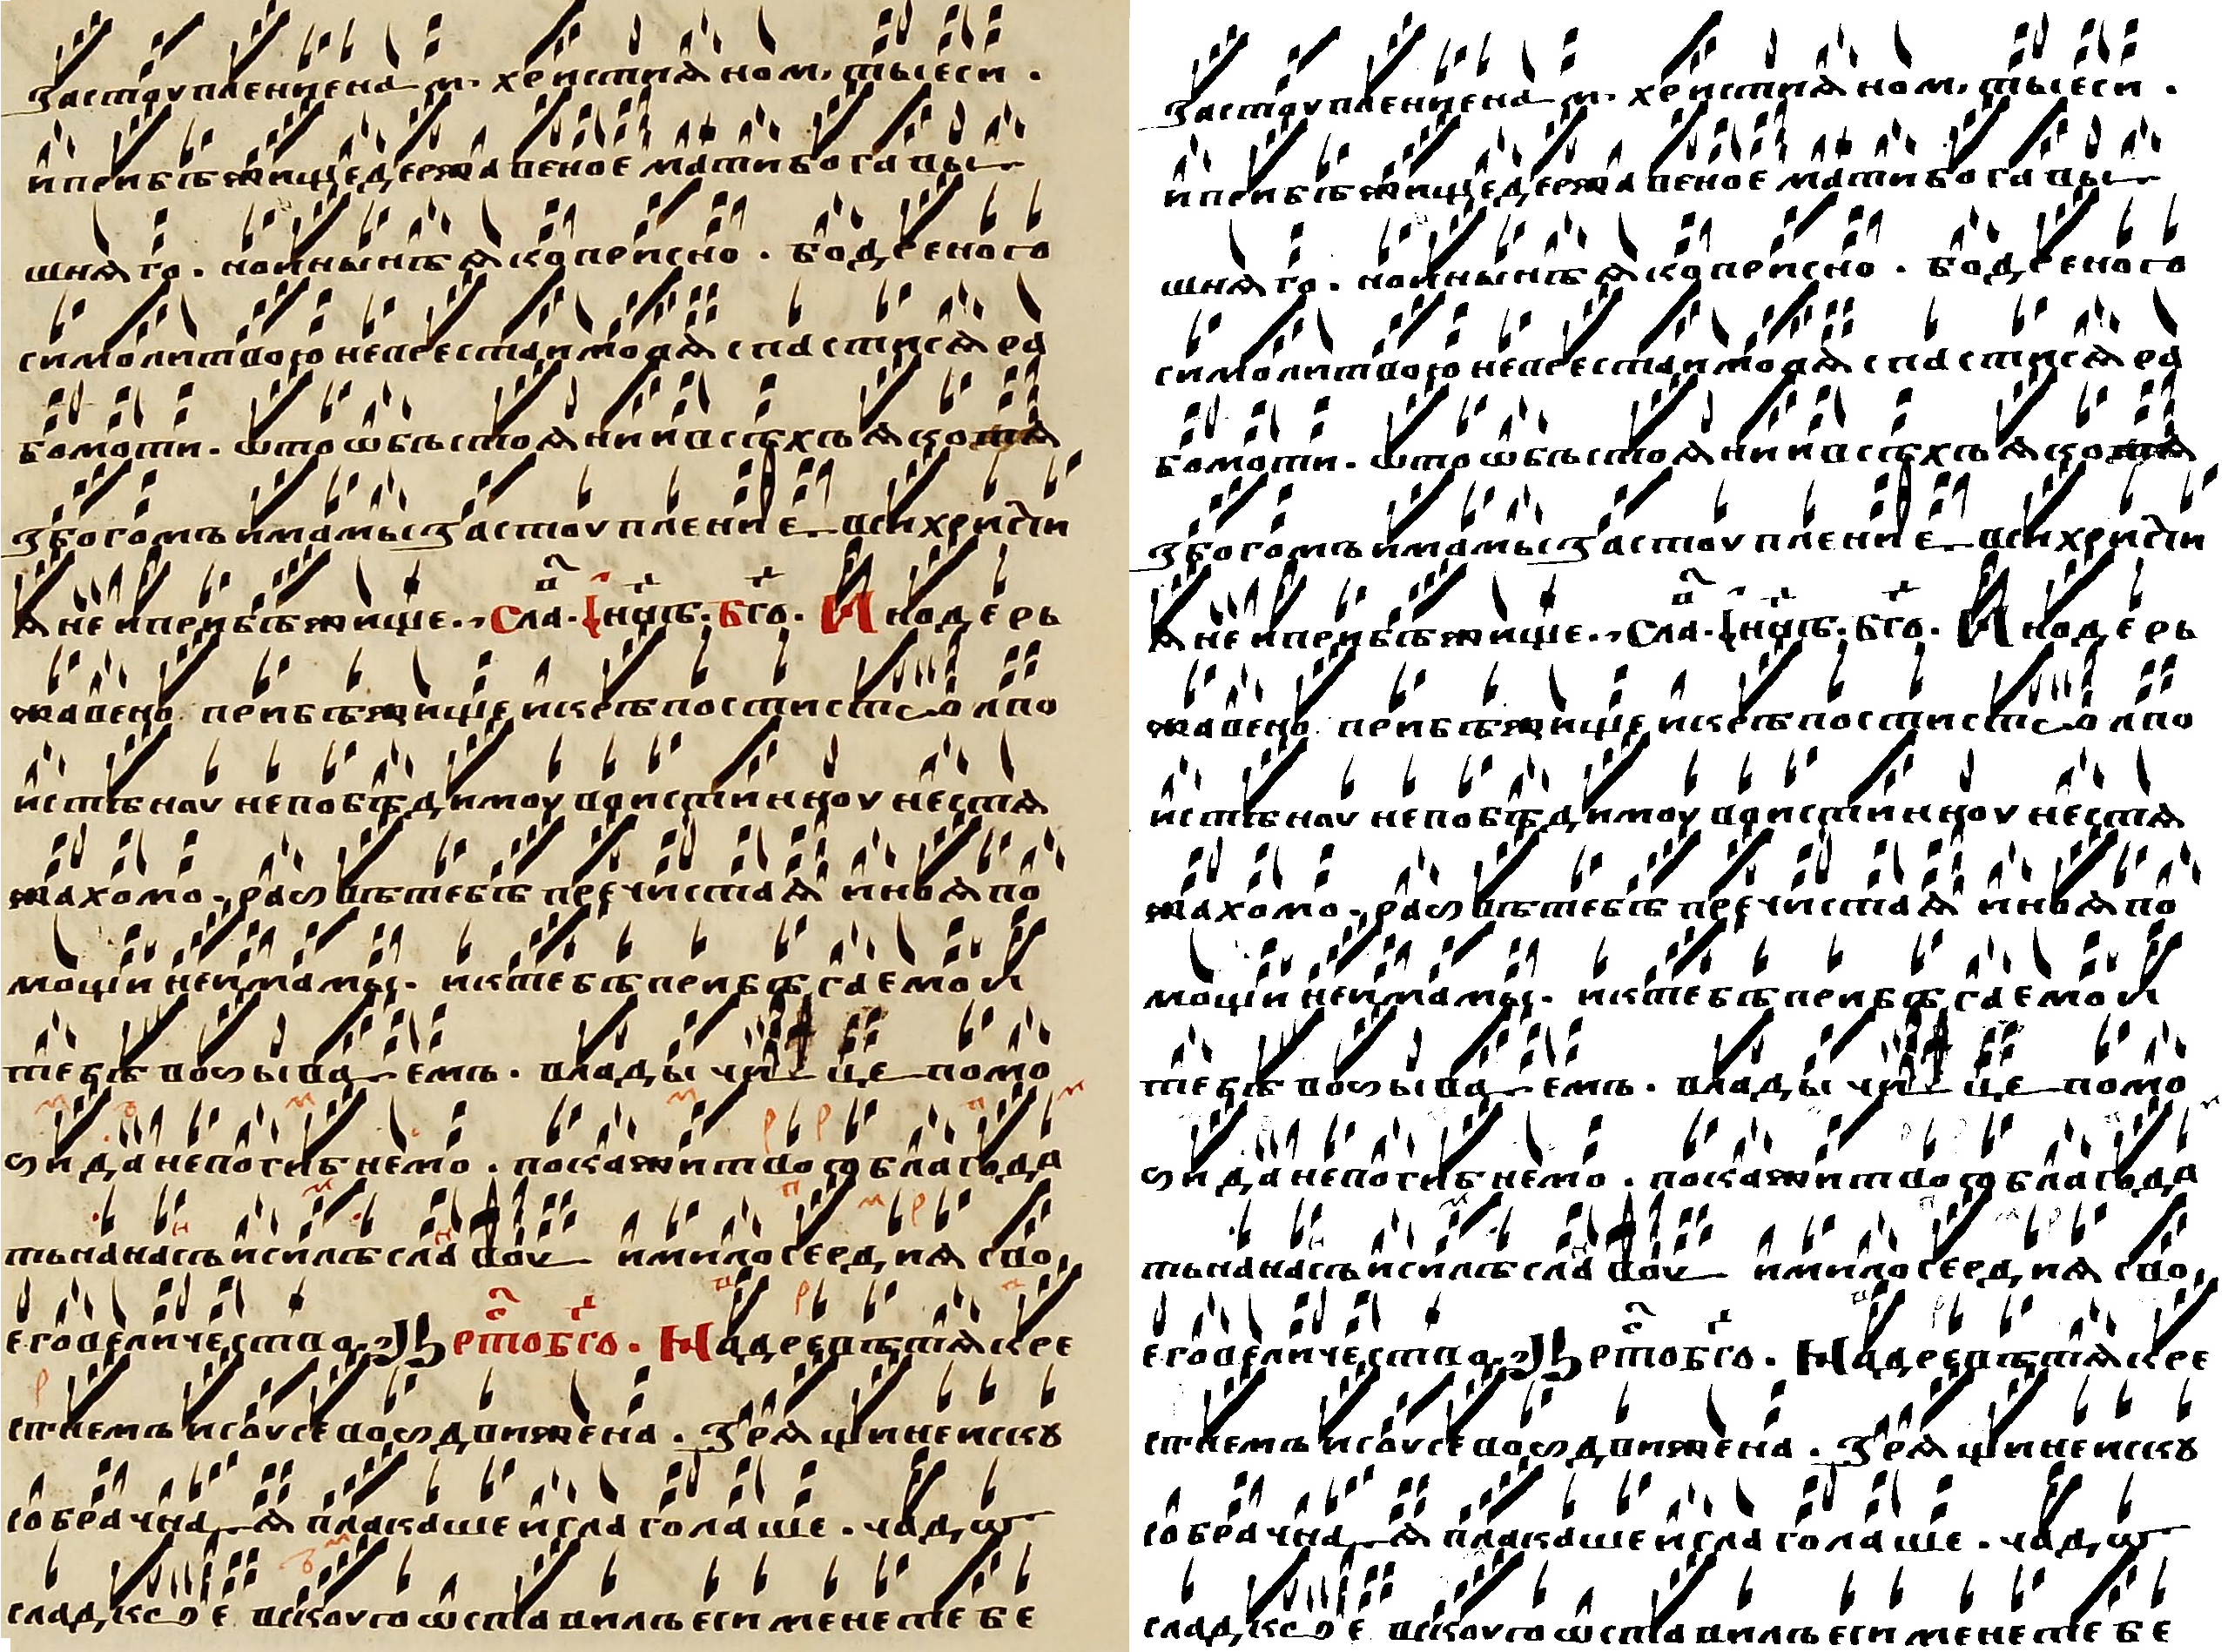
\includegraphics[width=.7\columnwidth]{./img/binaraize.png}%
  \end{center}
  \caption{Бинаризация страницы рукописи.}%
  \label{pic:binaraize}%
\end{figure}

После бинаризации осуществлялось выделение каждого крюка на странице, исправление шумов, их классификация, 
а также вырезка и сохранение полученных изображений. Из-за специфичности задачи и отсутствия автоматизированных 
инструментов для классификации крюков, сборка начальной выборки выполнялась вручную с использованием графического 
редактора Paint.net. (см. рис. \ref{pic:exaplesForSymbols}).
\begin{figure}[H]
  \begin{center}
    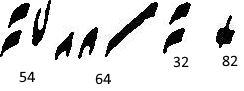
\includegraphics[width=.4\columnwidth]{./img/exaplesForSymbols.png}%
  \end{center}
  \caption{Пример нарезанных символов.}%
  \label{pic:exaplesForSymbols}%
\end{figure}


Итоговая статистика "чистых" символов: (см. рис. \ref{pic:exaplesForSymbols}).
\begin{figure}[H]
  \begin{center}
    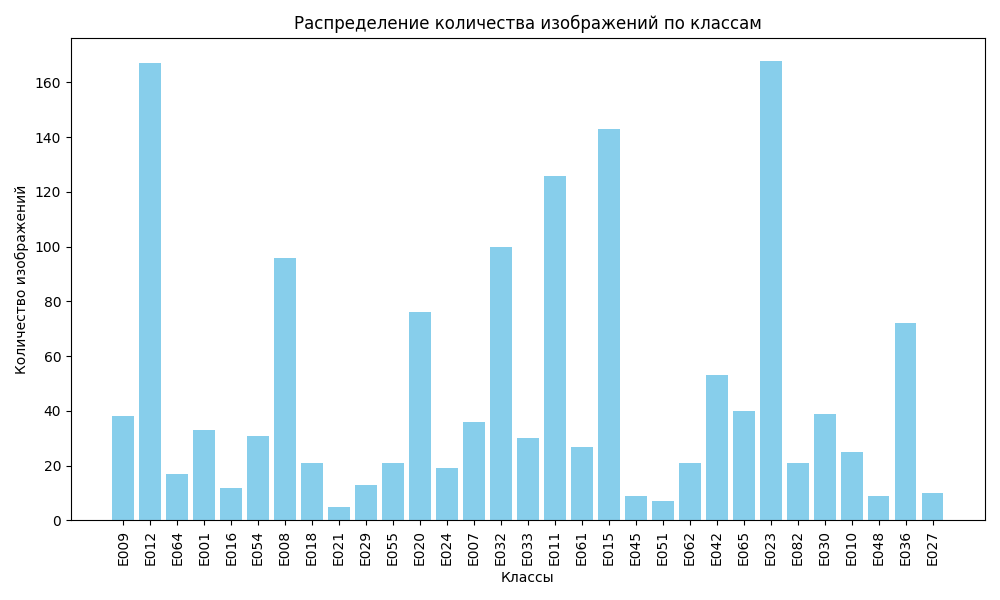
\includegraphics[width=.9\columnwidth]{./img/class_distribution.png}%
  \end{center}
  \caption{Статистика "чистых" символов.}%
  \label{pic:class_distribution}%
\end{figure}

В чистой статистике не учитываются крюки, которые встретились реже 10 раз, а также неопознанные, региональные особенности.
Общее же количество нарезанных крюков: 1686.

Для увеличения объема выборки применялось масштабирование крюков, что дополнительно обогатило данные различными 
вариантами размеров символов. (см. рис. \ref{pic:15_resampling}).
\begin{figure}[H]
  \begin{center}
    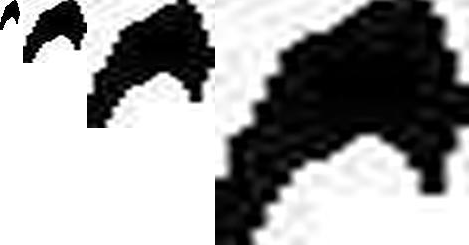
\includegraphics[width=.3\columnwidth]{./img/15_resampling.png}%
  \end{center}
  \caption{Пример мастабируемого 9-го символа.}%
  \label{pic:15_resampling}%
\end{figure}

Для повышения устойчивости модели к различным возможным искажениям, в выборку добавлялись крюки с шумами и размытием. 
Это позволяет модели лучше справляться с вариативностью данных при реальном использовании. (см. рис. \ref{pic:dirtyHook}).
\begin{figure}[H]
  \begin{center}
    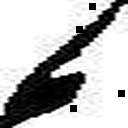
\includegraphics[width=.2\columnwidth]{./img/dirtyHook.png}%
  \end{center}
  \caption{Пример крюка с шумами.}%
  \label{pic:dirtyHook}%
\end{figure}


Для достижения равномерности выборки был рассчитан средний объём выборки для 90\% крюков. Недостаточно представленные классы были дополнительно уравновешены с использованием метода OverSampling.

Итоговая статистика по выборке: (см. рис. \ref{pic:itog}).
\begin{figure}[H]
  \begin{center}
    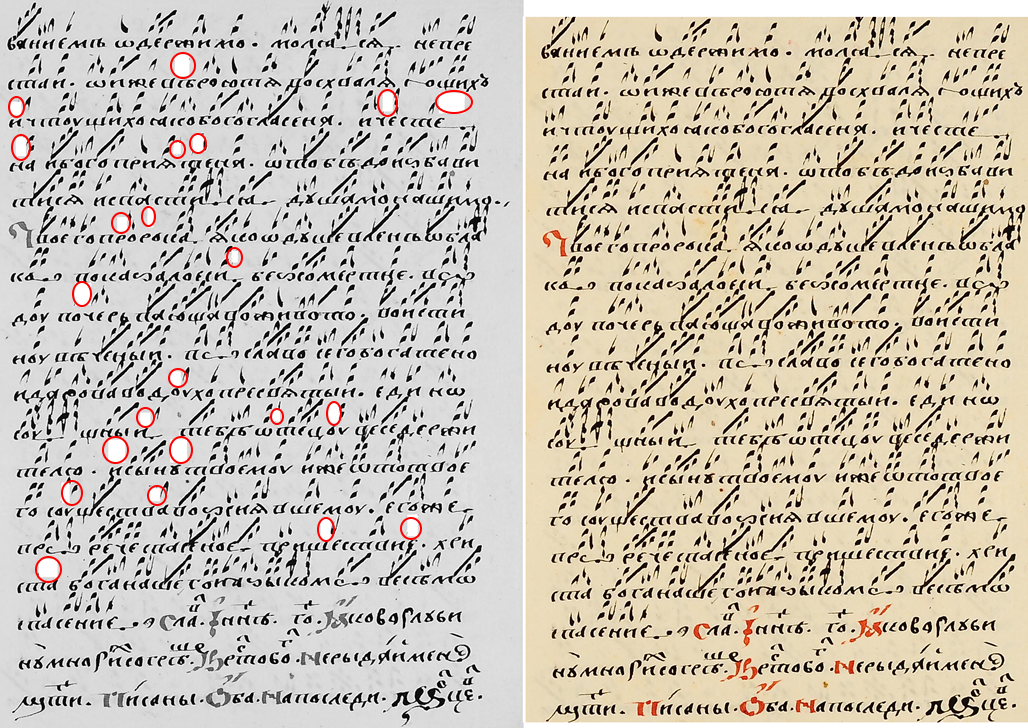
\includegraphics[width=.9\columnwidth]{./img/focusDetect.png}%
  \end{center}
  \caption{Итоговая статистика по выборке.}%
  \label{pic:itog}%
\end{figure}


\section{Выводы}
В ходе работы была сформирована обширная выборка, состоящая из 13 309 изображений крюков. 
Данная выборка сбалансирована и включает крюки различных размеров и качества изображений. 
На основе выборки будет обучаться нейросетевая модель для классификации и сегментации крюков и знамен.

%%% Local Variables:
%%% TeX-engine: xetex
%%% eval: (setq-local TeX-master (concat "../" (seq-find (-cut string-match ".*-3-pz\.tex$" <>) (directory-files ".."))))
%%% End:
